\documentclass{article}
\usepackage{graphicx}


\setlength{\parskip}{1em}

\begin{document}


\title{Resource Components}

Resource Components are ICE Components which contain a grid of visualization
resources. These resources can display files from a variety of sources,
such as CSV files or VisIt visualizations. Geometry and Mesh editors allow for
editing of shapes or meshes. All three can be added to an Item to offer
visualization of data.

\section{Prerequisites}

This tutorial assumes you will be making use of the sample classes in the
org.eclipse.ice.demo.visualization package for convenience. The two relevant
classes are VisualizationModel and VisualizationModelComplete. The former is an
example of a bare bones ICE Item, while the latter is the same class with all
the extra code required for the visualization components already added in.

If you are writing your own extension of ICE's Item class, then the same
principles can be used to add these components to it. See the New Item
Generation Tutorial, in the docs/newItemGeneration/ folder of the ICE repo for
details on how to create an Item.

\section{Adding the Components}

First, add the neccesary imports for the components being added to your Item. 

\begin{verbatim}
import java.io.IOException;
import org.eclipse.core.resources.IFile;
import org.eclipse.core.resources.ResourcesPlugin;
import org.eclipse.eavp.viz.modeling.ShapeController;
import org.eclipse.eavp.viz.modeling.ShapeMesh;
import org.eclipse.eavp.viz.modeling.base.BasicView;
import org.eclipse.ice.datastructures.form.GeometryComponent;
import org.eclipse.ice.datastructures.form.MeshComponent;
import org.eclipse.ice.datastructures.form.ResourceComponent;
import org.eclipse.ice.datastructures.resource.VizResource;
\end{verbatim}

Next, copy and paste the following example code into the end of your Item's
setupForm() method.

\begin{verbatim}
//Create the resource component
ResourceComponent resourceComponent = new ResourceComponent();

//Set the component's data members
resourceComponent.setName("Resources");
resourceComponent.setDescription("Results");
resourceComponent.setId(2);

//Declare the files and resources
VizResource csvResource = null;
VizResource visItResource = null;
IFile csvFile = null;
IFile visItFile = null;


//If the file was found, create the CSV resource and add it to the component
try{
			
	//Open the files
	csvFile = ResourcesPlugin.getWorkspace().getRoot().getProject("itemDB")
		.getFile("fib8.csv");
	visItFile = ResourcesPlugin.getWorkspace().getRoot().getProject("itemDB")
		.getFile("tire.silo");
			
	//If the file was found, create the CSV resource and add it to the component.
	if(csvFile.exists()){
		csvResource = new 
                    VizResource(csvFile.getLocation()
                    .toFile());
    	resourceComponent.addResource(csvResource);
	}
				        
	//If the file was found, create the VisIt resource and add it to 
	//the component
	if(visItFile.exists()){
		visItResource = new 
                    VizResource(visItFile.getLocation()
                    .toFile());
		resourceComponent.addResource(visItResource);
	}
}
catch(IOException e){
	e.printStackTrace();
}

//Create the geometry component
ShapeController geometryRoot = new ShapeController(new
    ShapeMesh(), new BasicView());
GeometryComponent geometryComponent = new 
    GeometryComponent();
geometryComponent.setGeometry(geometryRoot);

//Create mesh component
MeshComponent meshComponent = new MeshComponent();

//Add the components to the form
form.addComponent(resourceComponent);
form.addComponent(geometryComponent);
form.addComponent(meshComponent);	
		
//Set the context on the Form
form.setContext("visualization");
\end{verbatim} 

This code will add a Resource Component, Geometry Component, and Mesh Component
to your Item and load fib8.csv and tire.silo into the Resource Component.

You will also need to add the org.eclipse.ice.demo bundle to your operating
system's run configuration, as explained in the new item generation tutorial
(found in docs/newItemGeneration in the ICE repo). 


\section{Using the Resource Component}

\subsection{Establishing a VisIt Connection}

In order to visualize resources containing VisIt files, ICE must be connected to
a running VisIt installation. To set up this connection, select \texttt{Windows}
$\rightarrow$ \texttt{Preferences...} in ICE's menu bar. (On Mac OS X,
\texttt{Preferences} is instead located under \texttt{ICE} in the menu
bar.)

\begin{center}
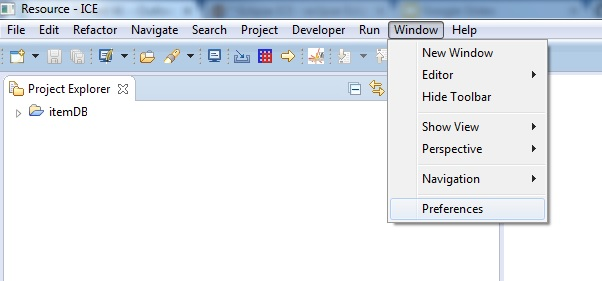
\includegraphics[width=12cm]{images/ICEPreferences}
\end{center}

Select \texttt{Visualization} $\rightarrow$ \texttt{VisIt} in the tree on the
left side of the \texttt{Preferences} window.

\begin{center}
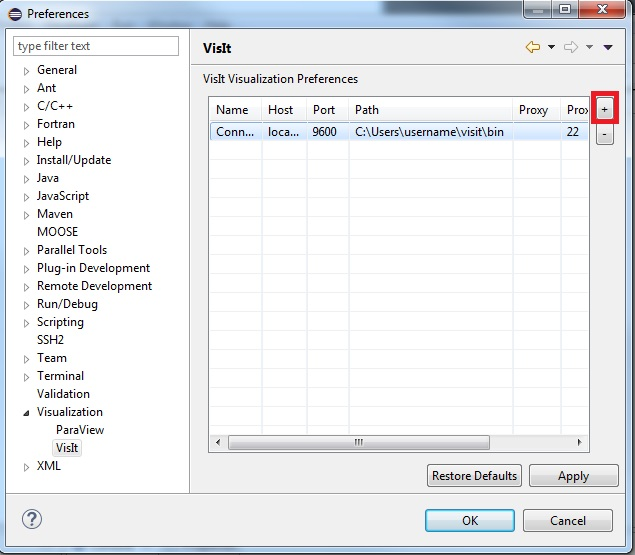
\includegraphics[width=12cm]{images/VisualizationPreferences}
\end{center}

Press the button with a "+" symbol in the upper right (highlighted in the image
above) to add a new row to the table. Click on the \texttt{Path} cell of the new
row and put the path of your installation of VisIt.

Press \texttt{Apply}, then \texttt{OK}, both in the lower right hand corner. ICE
will now open and connect to this VisIt installation each time ICE is opened.

\subsection{Opening Your Item}
Before opening your new Item, select the itemDB folder in the \texttt{Project
Explorer} and press the import button, highlighted below.

\begin{center}
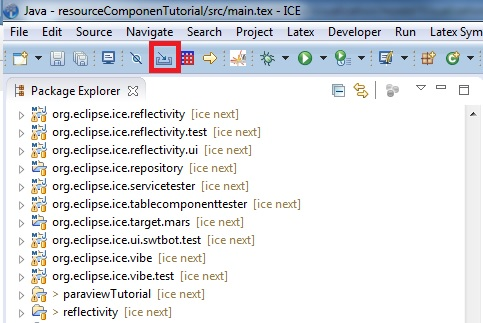
\includegraphics[width=12cm]{images/ImportButton}
\end{center}

Select the files you want to visualize and click OK. For the tutorial, these
should be the fib8.csv and tire.silo files from the USB drive's Data directory.
You should now see the two files within the itemDB folder.

Then select\texttt{New} $\rightarrow$ \texttt{Other\ldots} from the toolbar. In
the new dialog, select the \texttt{Create Item Wizard} and hit \texttt{Next}.
Then select the name of your Item and and press \texttt{Finish}. For the
tutorial, this will be Visualization Model. You can also select the
Visualization Model (Pre-completed) if you skipped the first part of the
tutorial.

Finally, switch to the ICE Perspective to ensure that the neccesary Views will
be open. To do this, click the \texttt{Open Perspective} button in the upper right
of the screen.

\begin{center}
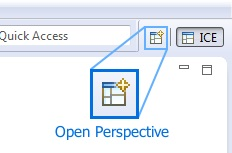
\includegraphics{images/ICE_OpenPerspective}
\end{center}

In the dialog, select \texttt{ICE} and press {OK}.

\subsection{Managing the Resources}

Your Item should look like this.

\begin{center}
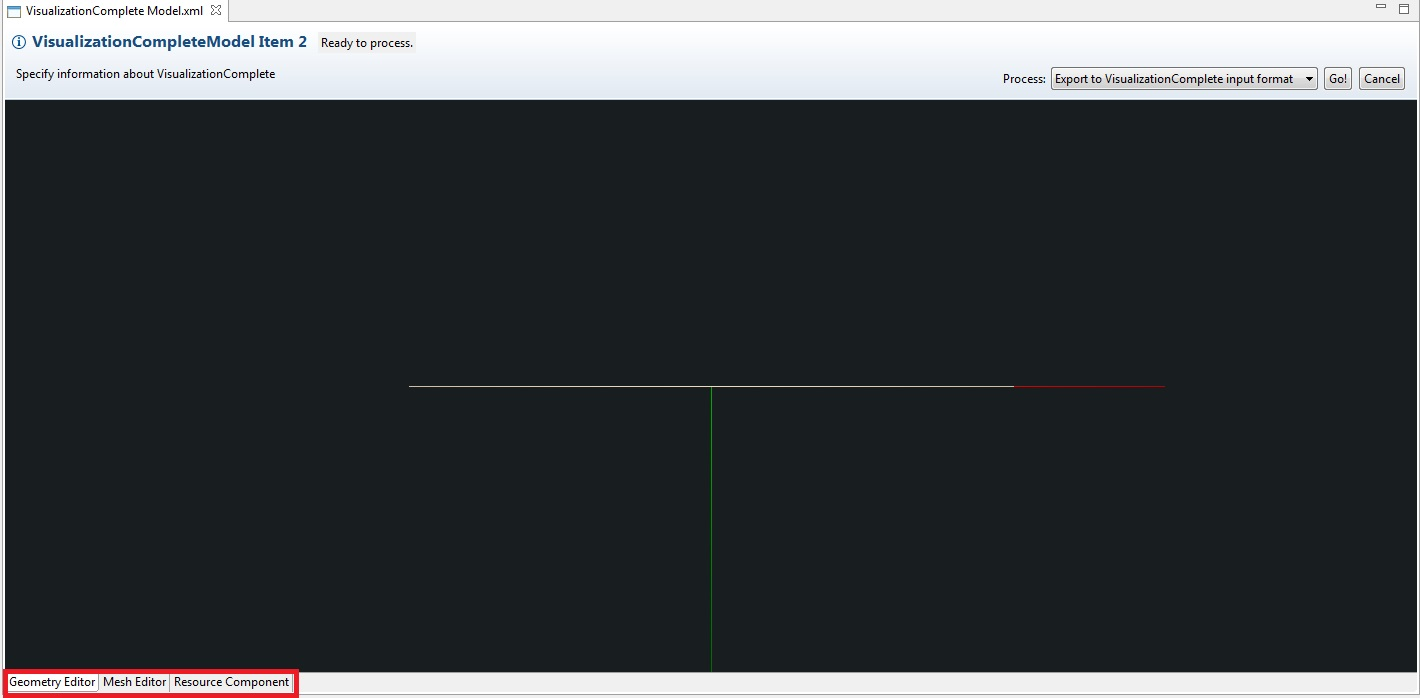
\includegraphics[width=12cm]{images/ItemTabs}
\end{center}

In the lower left are three tabs. Switch to the \texttt{Resource Component} tab
in your Item and to the \texttt{Resources} tab on the left, as shown below.

\begin{center}
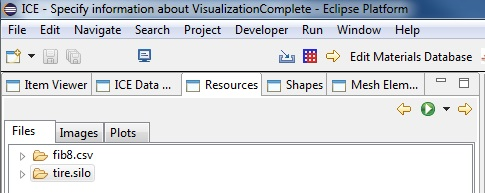
\includegraphics[width=12cm]{images/ResourcesTab}
\end{center}

Double click on both the file names to load them into the Resource Component.

At the top left of the screen will be controls for the component's layout.

\begin{center}
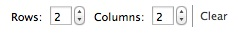
\includegraphics{images/ResourceComponentControls}
\end{center}

The \texttt{Clear} button will close all plots in the component. The other two
controls will allow you to specify the number of rows and columns in the grid.
Be careful when reducing them, as any plots which no longer fit in the grid will
be closed.

If you hover over a plot, a button will appear in the upper left hand corner.
Clicking it will close that plot. 

\begin{center}
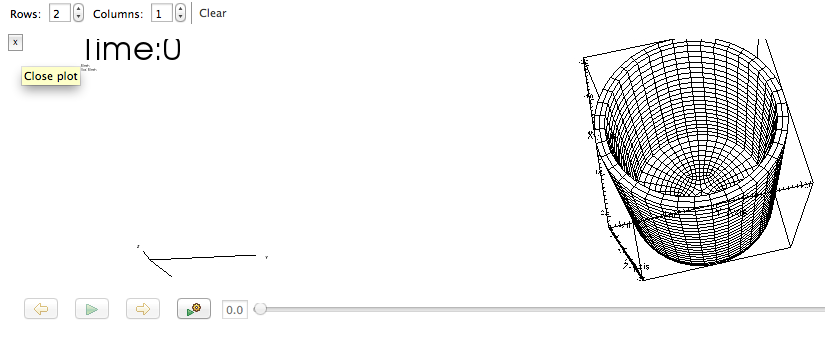
\includegraphics[width=12cm]{images/ClosePlotButton}
\end{center}

\subsection{Interacting with VisIt Plots}

\begin{center}
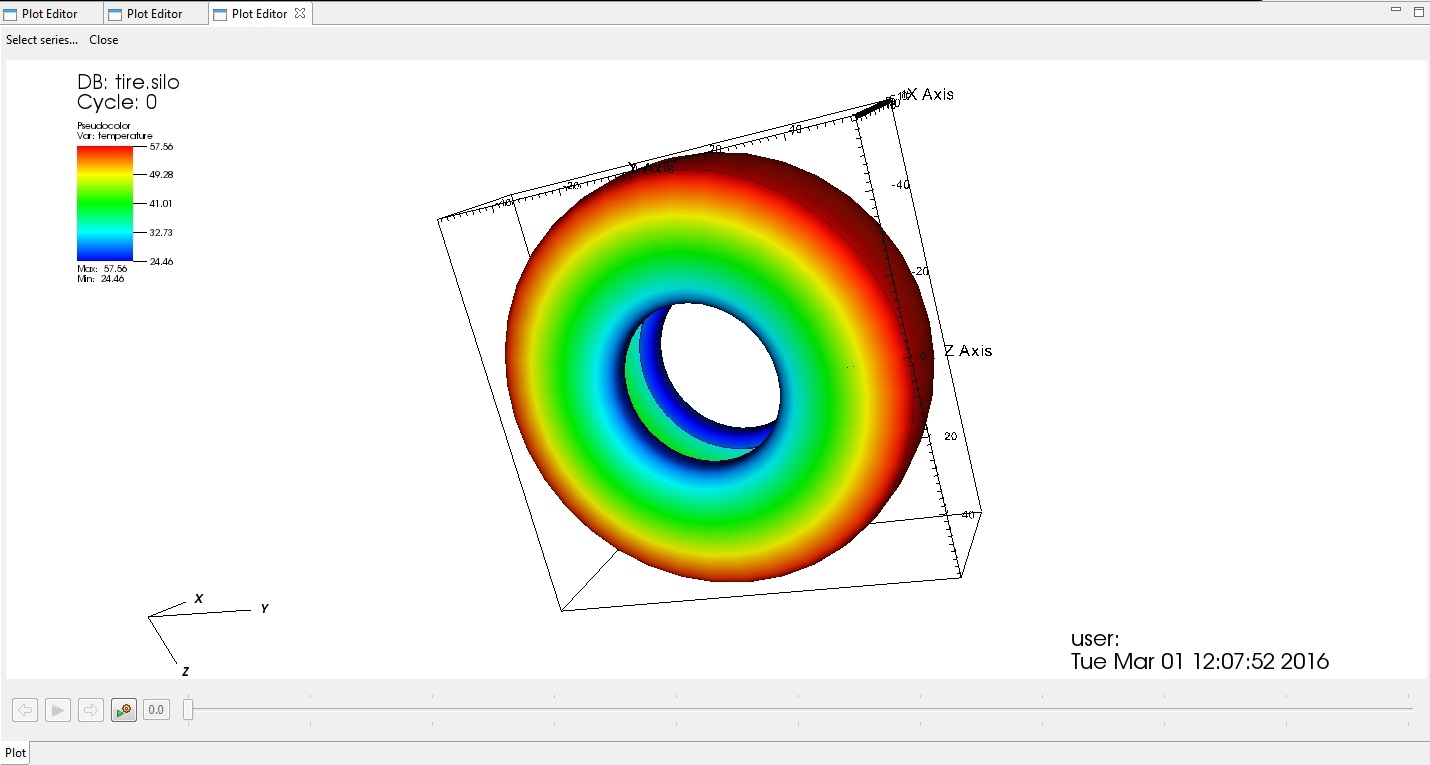
\includegraphics[width=12cm]{images/VisItPlot}
\end{center}

A VisIt plot will contain a 3D visualization of some model. You can click and
drag within the plot to rotate the image and zoom by scrolling your mouse wheel.
Right clicking in the plot will open a context menu, providing options for how
the model will be displayed.

At the bottom of the plot will be a series of controls for animation. If your
plot does not have time series data, they will be greyed out. 

\begin{center}
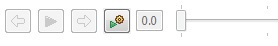
\includegraphics[width=12cm]{images/TimeSliderWidget} 
\end{center}

The plot can be set to display an arbitrary time step by either dragging the
slider or by typing a time into the box to its left.

\subsection{Interacting with CSV Plots}

\begin{center}
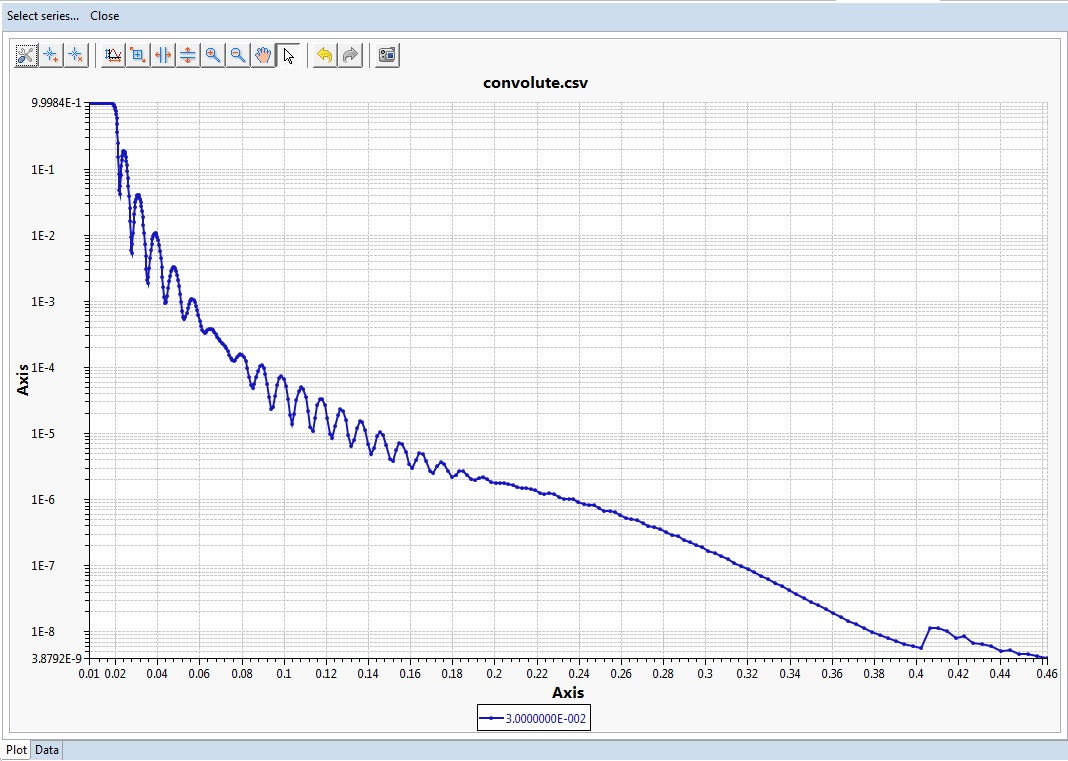
\includegraphics[width=12cm]{images/CSVGraph}
\end{center}

The top of the CSV plot has a row of buttons which control various aspects of
the graph's presentation. Right clicking will open a context menu allowing you
to choose which of the available series to plot.

\subsection{Editing 3D Structures}

ICE also contains capabilities to render graphics with the Geometry Editor and
Mesh Editor. Programatically populating these editors with custom input is
beyond the scope of this tutorial. However, what follows will be a brief
overview of the editors' functionality.

\subsubsection{The Geometry Editor}

Now switch to the \texttt{Geometry Editor} tab in your Item and the
\texttt{Shapes} tab on the left.

Clicking the \texttt{Add Primitives} button will display a drop down of
primitive shapes which can be added to the scene.

\begin{center}
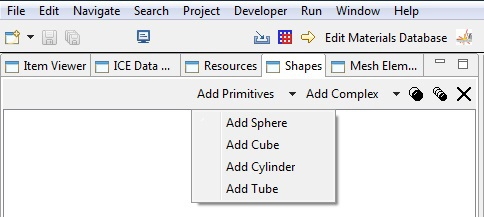
\includegraphics[width=12cm]{images/AddPrimitiveShape}
\end{center}

Complex shapes can similarly be added using the \texttt{Add Complex} button.

\begin{center}
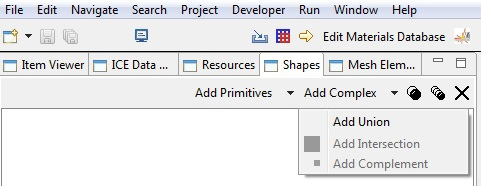
\includegraphics[width=12cm]{images/AddComplexShape}
\end{center}

Primitive shapes can be added under complex shapes by selecting anything beneath
the desired parent complex shape before adding the new primitive.

\begin{center}
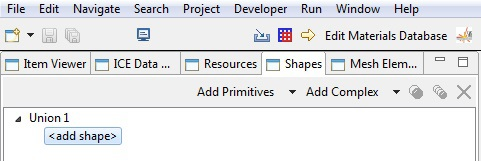
\includegraphics[width=12cm]{images/ComplexShapeTree}
\end{center}

The three other buttons are responsible for creating copies of or removing
selected shapes from the tree. 

The Transformation View, in the lower left, has spaces to set the rotation, scale, 
and translation of a selected object.

\begin{center}
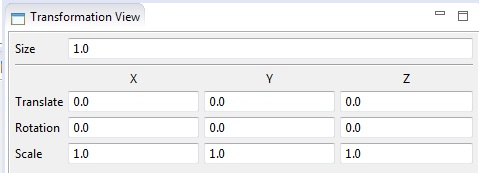
\includegraphics[width=12cm]{images/TransformationView}
\end{center}

\subsubsection{The Mesh Editor}

Now switch to the \texttt{Mesh Editor} tab in your Item and \texttt{Mesh
Elements} tab on your left.

Clicking within the grid will create a vertex, until the fourth completes the
polygon.

\begin{center}
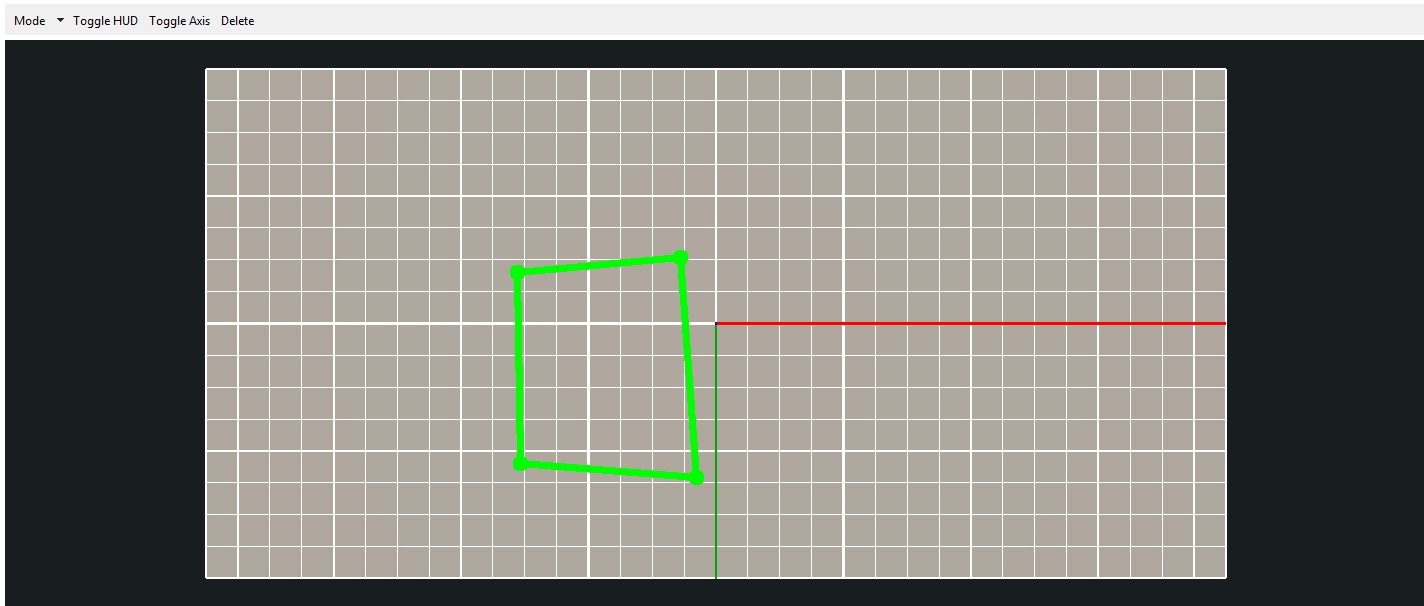
\includegraphics[width=12cm]{images/AddPolygon}
\end{center}

Click again to make the polygon permanent, signified by turning purple, or hit
\texttt{Esc} to cancel.

\begin{center}
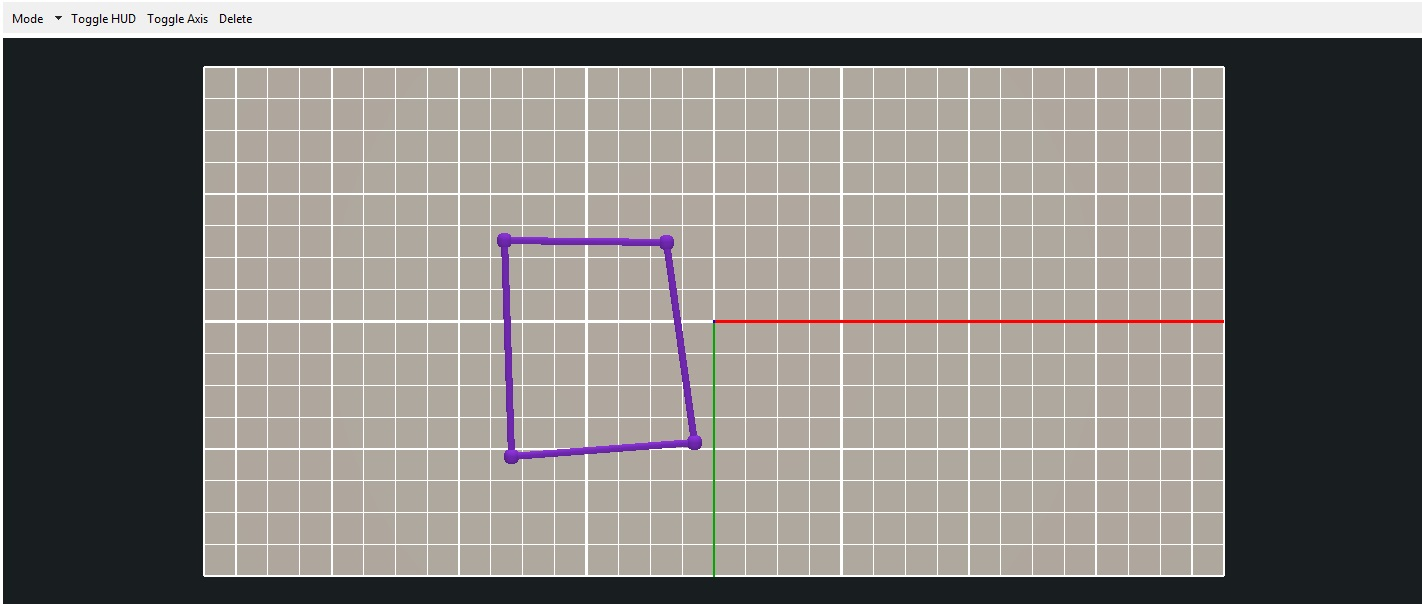
\includegraphics[width=12cm]{images/NewPolygon}
\end{center}

The \texttt{Mode} button in the top left allows you to switch between
\texttt{Add Elements} mode, used previously, and \texttt{Edit Elements} mode.

\begin{center}
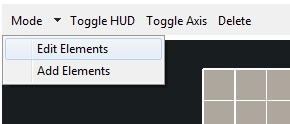
\includegraphics[width=12cm]{images/EditMode}
\end{center}

In edit mode, you can click a vertex (or vertices) to select them. 

\begin{center}
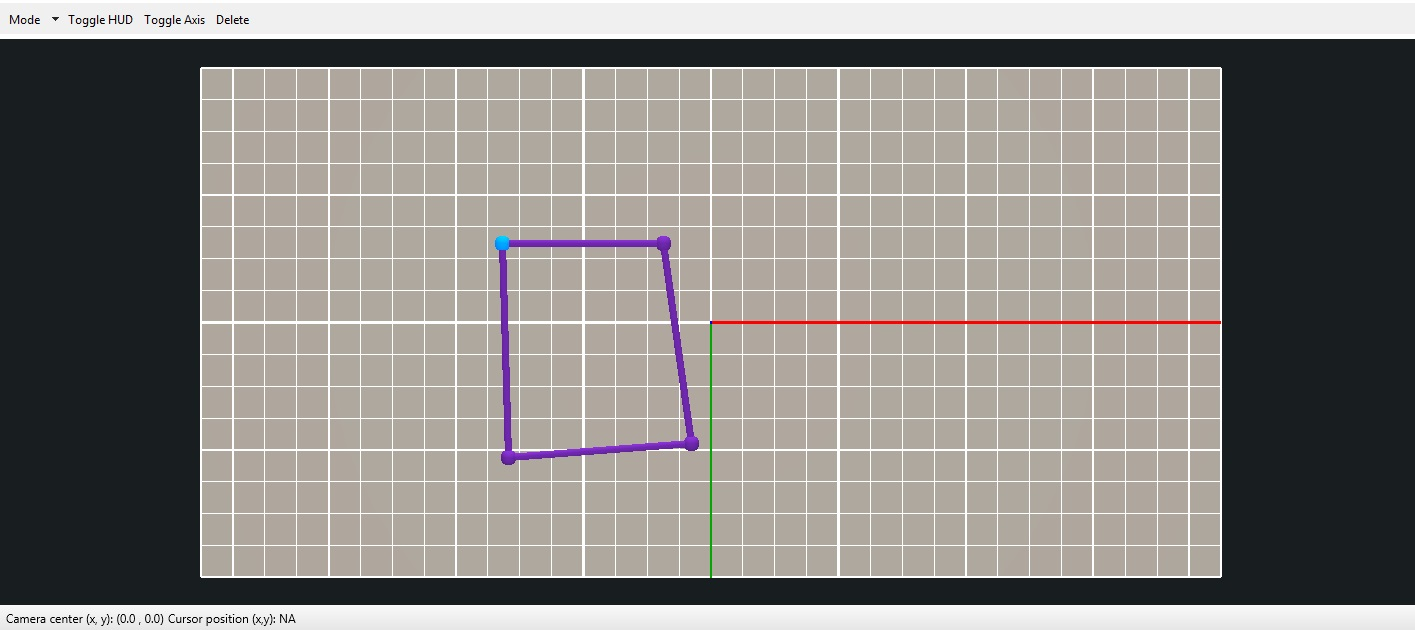
\includegraphics[width=12cm]{images/SelectedVertex}
\end{center}

You can click and drag a vertex to move all selected vertices around the grid.

\section{Further Reading}

This tutorial has only given a brief overview of the ways in which you can use
ICE's visualization tools. For more detailed information, look under the
\texttt{docs} folder in the ICE repository. The visualization folder contains a
tutorial on the CSV and VisIt plots, while the geometryEditor and meshEditor
folders have tutorials on the geometry and mesh editors, respectively. 

\end{document}
